\documentclass[english]{beamer}
\usepackage[english,activeacute]{babel}
%\usepackage[utf8]{inputenc}
\usepackage{inputenc}
\usepackage{listings}
\usepackage{xcolor}
\usepackage{tikz}
\usepackage{caption}
\usepackage{amsmath}
\usepackage{amssymb}
\usepackage{breqn}

\definecolor{red}{RGB}{255,20,0}
\definecolor{green}{RGB}{0,255,0}
\definecolor{dgreen}{RGB}{118,151,53}
\definecolor{blue}{RGB}{2,103,255}
\definecolor{oran}{RGB}{255,93,0}

\newcommand{\blue}{\textcolor{blue}}
\newcommand{\red}{\textcolor{red}}
\newcommand{\green}{\textcolor{green}}
\newcommand{\dgreen}{\textcolor{dgreen}}
\newcommand{\oran}{\textcolor{oran}}
\newcommand{\gray}{\textcolor{gray}}
\newcommand{\soft}{\textcolor{gray}}
\definecolor{gray97}{gray}{.97}
\definecolor{gray75}{gray}{.75}
\definecolor{gray45}{gray}{.45}
%\setbeamercolor{block body}{bg=white, fg=black}


\newcommand{\nbody}{$N-$body}
\newcommand{\GR}{{\sc Gravidy }}

\newcommand{\bs}{\boldsymbol}

\renewcommand\mathfamilydefault{\rmdefault}
\setbeamertemplate{blocks}[rounded][shadow=true]

%\usetheme{simplebeauty}

\lstset{frame=Ltb,
     framerule=0pt,
     aboveskip=0.5cm,
     framextopmargin=3pt,
     framexbottommargin=3pt,
     framexleftmargin=0.4cm,
     framesep=0pt,
     rulesep=.4pt,
%     backgroundcolor=\white,
     rulesepcolor=\color{white},
     %
     stringstyle=\ttfamily,
     showstringspaces = false,
     basicstyle=\tiny\ttfamily,
     %commentstyle=\color{gray45},
     %keywordstyle=\bfseries,
     %
     numbers=left,
     numbersep=13pt,
     numberstyle=\tiny,
     numberfirstline = false,
     breaklines=true,
     emph = {[1]\_\_device\_\_,\_\_global\_\_,\_\_syncthreads,pthread\_create,pthread\_join,pragma,omp,parallel,private, threadIdx, blockDim, blockIdx,cudaThreadSynchronize, while, total, MPI_Allreduce},
     emphstyle={[1]\color{blue}},
   }

% minimizar fragmentado de listados
\lstnewenvironment{listing}[1][]
   {\lstset{#1}\pagebreak[0]}{\pagebreak[0]}

\lstdefinestyle{consola}
   {basicstyle=\scriptsize\bf\ttfamily,
    backgroundcolor=\color{gray75},
   }
\lstdefinestyle{C}
   {language=C,
   }



\author[C. Maureira-Fredes]
       {\large Cristián Maureira-Fredes}
\title[HPC DSS]
      {\huge HPC for Dense Stellar Systems}
\institute[AEI]
          {Albert Einstein Institute}

\begin{document}

%\bibliographystyle{unsrt}

% First slide
\begin{frame}[t,plain]
    \titlepage
\end{frame}

\begin{frame}
    \frametitle{Contents}
    \tableofcontents
\end{frame}

\section{Introduction}

\begin{frame}
    \frametitle{Introduction}
    \framesubtitle{Motivation (1/2)}

    \begin{columns}
        \begin{column}{0.6\textwidth}
            \begin{itemize}
                \item Dynamical evolution of a dense stellar systems.
                      ({\nbody} Problem)
                \item Newtonian systems compounded by \blue{more than two stars},
                      needs numerical approaches.
            \end{itemize}
        \end{column}
        \begin{column}{0.4\textwidth}
            \begin{figure}
                \centering
                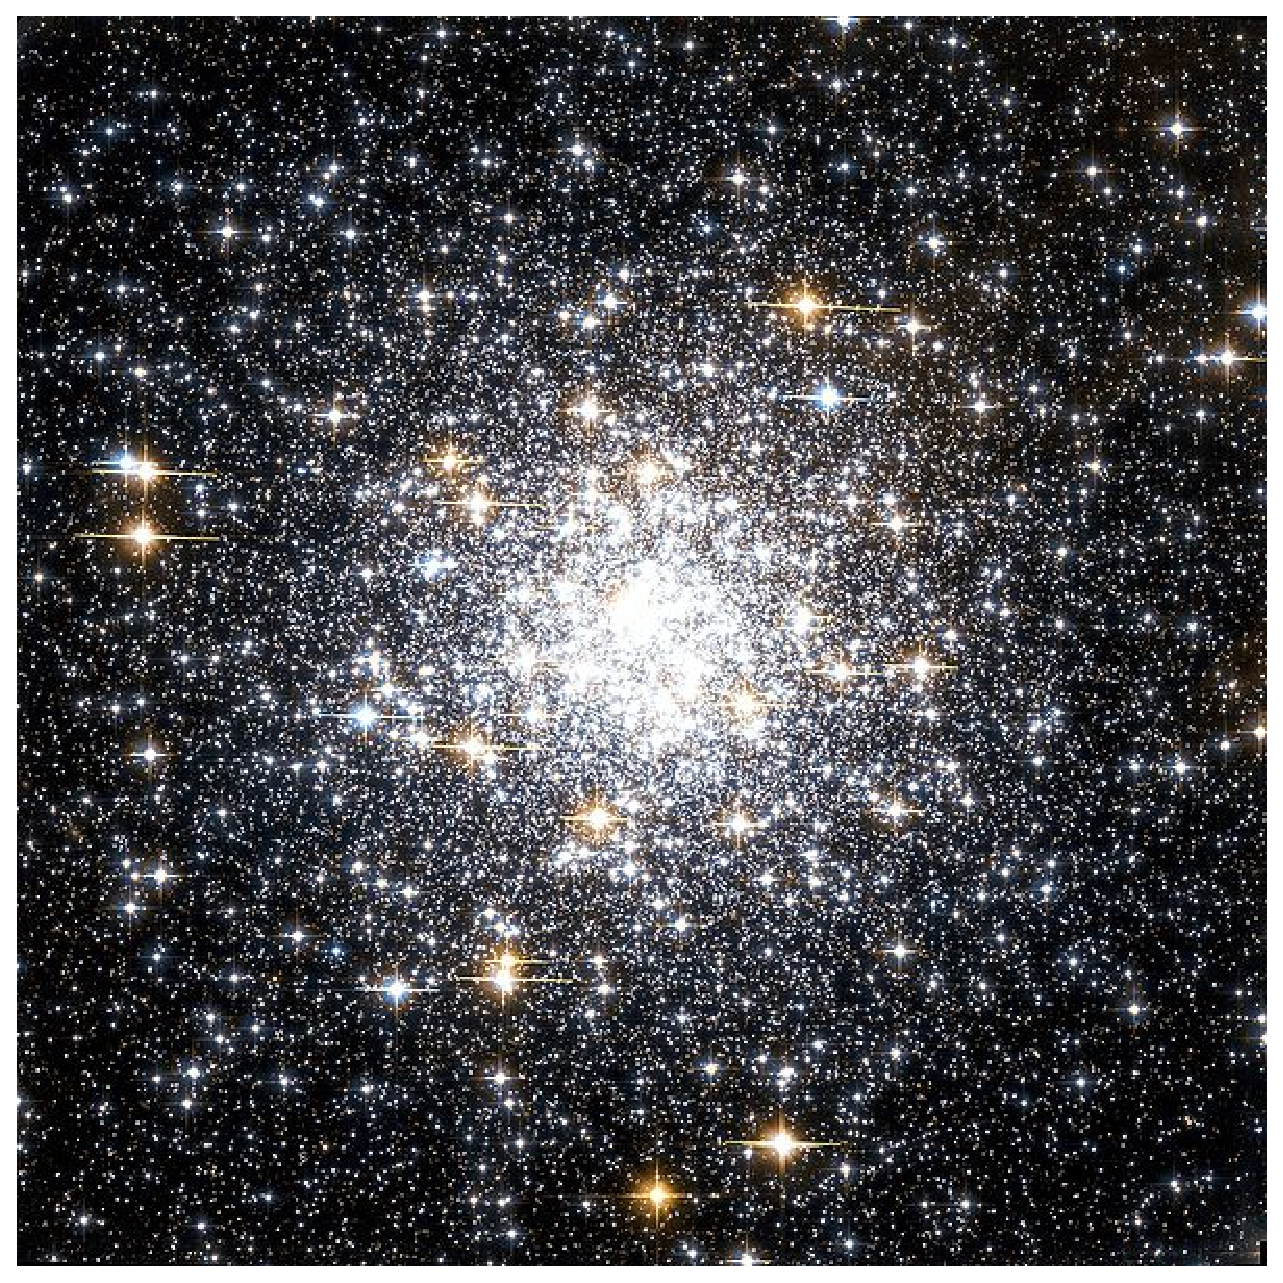
\includegraphics[width=0.8\textwidth]{img/m69}
                \caption{Globular cluster ``Messier 69'' in the constellation Sagittarius.}
                \label{fig:m69}
            \end{figure}
        \end{column}
    \end{columns}
\end{frame}

\begin{frame}
    \frametitle{Introduction}
    \framesubtitle{Motivation (2/2)}

    \begin{columns}
        \begin{column}{0.5\textwidth}
            \begin{itemize}
                \item Evolution of the High Performance Computing (HPC).
            \end{itemize}
            \begin{center}
                \includegraphics[width=0.8\textwidth]{img/top500}
            \end{center}
        \end{column}
        \begin{column}{0.5\textwidth}
            \begin{figure}
                \centering
                \includegraphics[width=0.8\textwidth]{img/cluster}
                \caption{GPU Cluster Mole-8.5 in Beijing, at the Institute of Process
                         Engineering of Chinese Academy of Sciences.
                         (372 nodes and 2,000 NVIDIA Fermi C2050 GPUs)}
                \label{fig:m69}
            \end{figure}
        \end{column}
    \end{columns}
\end{frame}

\section{The {\nbody} problem}
\begin{frame}
    \frametitle{The {\nbody} problem}
    \framesubtitle{Definition}

    Purely dynamic problem, in which the bodies orbital evolution
    is determined exclusive by the \blue{gravitational interaction},

    \begin{align}
        \bs{\ddot{r}}_{i} &= -G \sum\limits^{N}_{\substack{j=1\\j\neq i}}
                              m_{j} {(\bs{r}_i - \bs{r}_j)\over
                              | \bs{r}_i - \bs{r}_j|^{3}}\label{eq:nbody},
    \end{align}

    \noindent
    where $G$ is the gravitational constant
    ($6.67384\times 10^{-11} m^{3} kg^{-1} s^{-2}$),
    $m_j$ is the mass of the $j$th particle
    and $\bs{r}_j$ the position in \emph{Cartesian} coordinates.
    \begin{block}{\red{Note}}
        We denote vectors by bold fonts.
    \end{block}
\end{frame}


\begin{frame}
    \frametitle{The {\nbody} problem}
    \framesubtitle{Checking the system evolution}

    \begin{itemize}
        \item The \blue{initial condition} are usually the masses,
            position and velocity.

        \item \blue{Chaotic nature}, the evolution of this systems
         will depend of the initial parameters.

        \item The often invariant to check the integration of the system,
            is the system's \blue{energy},

            \begin{align}
                E &= {1 \over 2} \sum\limits^{N}_{i=1} m_{i} \bs{v}_{i}^{2} -
                     \sum\limits_{i=1}^{N} \sum\limits_{j > i}^{N}
                     {G m_{i} m_{j} \over |\bs{r}_{i} - \bs{r}_{j}|},
            \end{align}

            \noindent
            where $\bs{v}_i$ is the velocity of the particle $i$.
    \end{itemize}

\end{frame}


\begin{frame}
    \frametitle{The {\nbody} problem}
    \framesubtitle{Particle's time steps}

    \begin{itemize}
        \item The real scenario, \blue{individual} time steps.
        \begin{itemize}
            \item \red{Hard} scenario for parallel computing.
        \end{itemize}
        \item Forming groups of particles, \blue{block} time steps scheme~\cite{Press86}.
        \begin{itemize}
            \item  This time step scheme is popular among  {\nbody} code,
                like Starlab~\cite{portegies2001, hut2003}, Aarseth {\nbody}
                codes~\cite{Aarseth99, Aarseth03,NitadoriAarseth2012},
                $\phi$GRAPE~\cite{harfst2008},
                which gives us the possibility to check our algorithm behavior.
        \end{itemize}
    \end{itemize}
\end{frame}


\begin{frame}
    \frametitle{Introduction}
    \framesubtitle{{\nbody} algorithms classification}

    \begin{description}
        \item[Collision-less]
            A star just sees the \blue{background potential} of the rest of
            the stellar system.
            A model of this situation is the Barnes-Hut Treecode
            with a complexity $O(N\log N)$~\cite{BarnesHut86}
            or the fast multipole method with $O(N)$~\cite{GreendardThesis}.
            \vspace{0.7cm}
        \item[Collisional (``direct-summation'')]
            One star integrates \blue{all gravitational forces}
            for all stars. This typically scale as $O(N^{2})$.
            A well-known example is the family of algorithm of Aarseth
            the direct-summation {\sc Nbody} integrator~\cite{Aarseth99,Spurzem1999,Aarseth03}
            or {\sc kira} code~\cite{PortegiesZwartEtAl01}.
    \end{description}

\end{frame}

\section{Computational aspects}
\begin{frame}
    \frametitle{Introduction}
    \framesubtitle{The computational challenge}

    \begin{itemize}
        \item The {\nbody} codes evolution is related to the available
                \blue{hardware} in our time.
        \item The algorithms with a complexity of $O(N^{2})$ or $O(N^{3})$ require
                \red{supercomputers}.
        \begin{itemize}
            \item  e.g \blue{beowulf clusters},
                which require a parallelization of the code
                ({\sc Nbody6++} developed by Spurzem et al.~\cite{Spurzem1999}).

            \item Special-purpose hardware, like the \blue{GRAPE} (short for GRAvity
                PipE system~\cite{TMFES96,MT98,Makino98,GRAPE6A}.

        \end{itemize}

        \item  The literature overview reveals a strong interest on porting the existing codes to the
            \blue{GPU} architecture, like e.g. the work
            of~\cite{Portegies2007a,Hamada2007,Belleman2008}
            on single nodes or using large
            clusters~\cite{berczik2011high,NitadoriAarseth2012,Capuzzo-DolcettaEtAl2013}.

    \end{itemize}

\end{frame}

\subsection{GPU Computing}
\begin{frame}
    \frametitle{Introduction}
    \framesubtitle{GPU Computing}

    \begin{columns}
        \begin{column}{0.6\textwidth}
            \begin{itemize}
                \item \emph{``Using a GPU (Graphic Processing Unit) together with
                      a CPU to accelerate scientific calculation operations
                      or general purpose calculation''}
            \end{itemize}
        \end{column}
        \begin{column}{0.4\textwidth}
             \begin{figure}
                 \centering
                 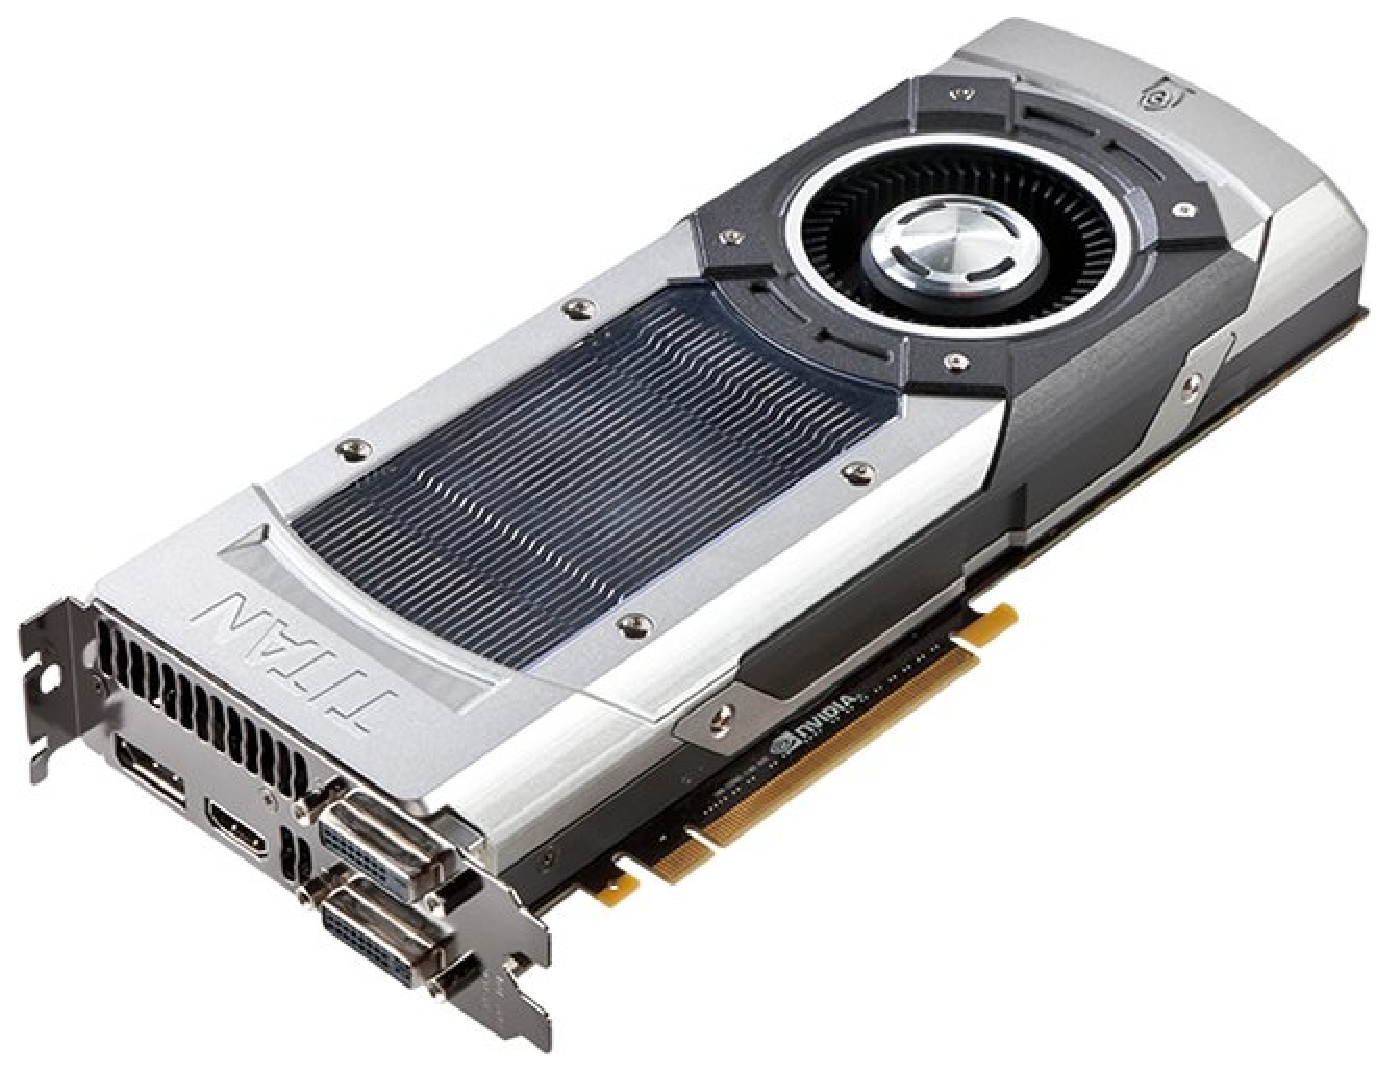
\includegraphics[width=0.8\textwidth]{img/titan}
                 \caption{NVIDIA\textsuperscript{\textregistered} GTX Titan}
                 \label{fig:titan}
             \end{figure}
        \end{column}
    \end{columns}
\end{frame}

\begin{frame}
    \frametitle{Introduction}
    \framesubtitle{CPU/GPU Design}

    \begin{itemize}
        \item CPU,
        \begin{itemize}
            \item Designed to have a good \blue{performance}
                  in parallel and non-parallel scenarios.
            \item Minimizes the \blue{latency} experimented by a thread
                  (large cache memory)
        \end{itemize}
        \item GPU,
            \begin{itemize}
            \item Designed to perform highly parallel work.
            \item Maximizes the \blue{throughput} of all the threads.
            \end{itemize}
    \end{itemize}

    \begin{footnotesize}
        \begin{columns}
            \begin{column}{0.35\textwidth}
            \begin{block}{Performance}
                Capacity of perform individual instructions in a certain time.
            \end{block}
            \end{column}
            \begin{column}{0.3\textwidth}
            \begin{block}{Latency}
                Measure of time delay experienced in a system.
            \end{block}
            \end{column}
            \begin{column}{0.3\textwidth}
            \begin{block}{Throughput}
                Capacity of perform a whole task in a certain time.
            \end{block}
            \end{column}
        \end{columns}
    \end{footnotesize}

    %\begin{description}
    %    \item[Performance]
    %            Capacity of perform individual instructions in a certain time.
    %    \item[Throughput]
    %            Capacity of perform a whole task in a certain time.
    %    \item[Latency]
    %            Measure of time delay experienced in a system.
    %    \item[Granularity]
    %            Break down a system into small parts.(Coarse and Fine)
    %\end{description}
\end{frame}

\begin{frame}
    \framesubtitle{Introduction}
    \frametitle{GPU Architecture}

    \begin{columns}
        \begin{column}{0.5\textwidth}
            \begin{block}{Task parallelism}
                Each processor perform a different task.
            \end{block}
            \begin{block}{Data parallelism}
                Each processor perform the same task, but not on the same data set.
            \end{block}
        \end{column}
        \begin{column}{0.5\textwidth}
             \begin{figure}
                 \centering
                 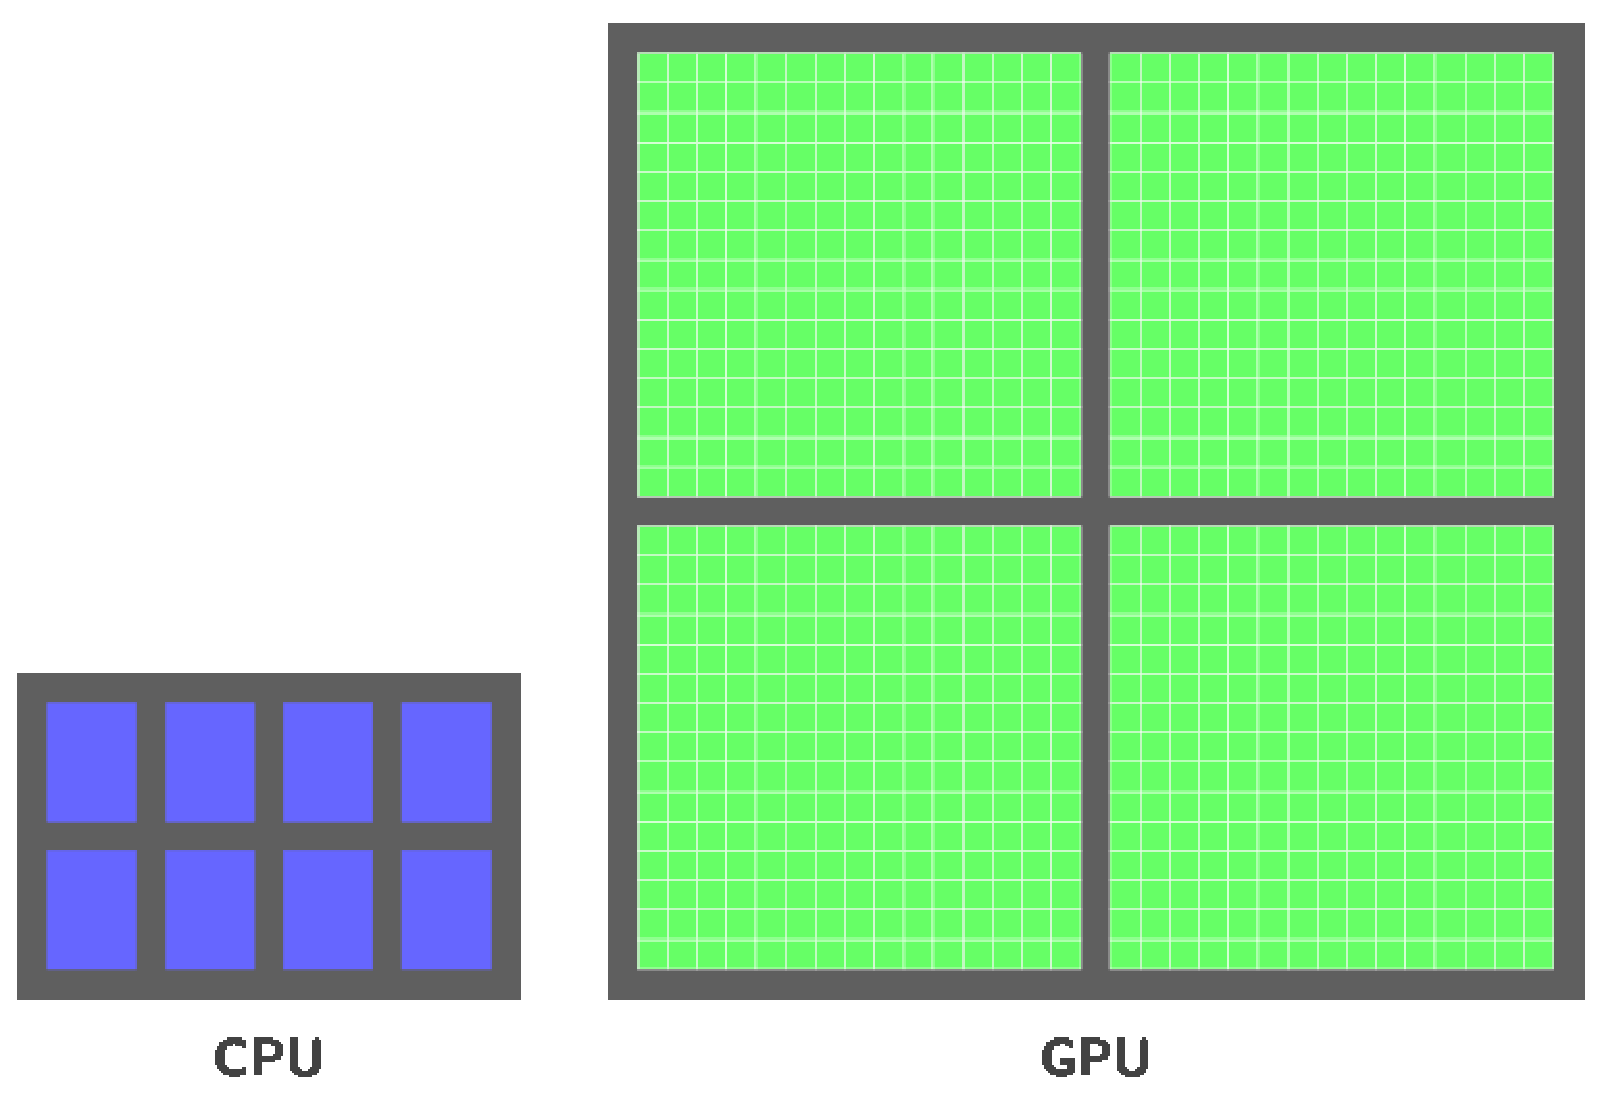
\includegraphics[width=0.8\textwidth]{img/cpu_gpu}
                 \caption{GPU and CPU core scheme}
                 \label{fig:titan}
             \end{figure}
        \end{column}
    \end{columns}
\end{frame}

\subsection{Programming strategy}
\begin{frame}
    \frametitle{Introduction}
    \framesubtitle{Programming strategy}

    \begin{columns}
        \begin{column}{0.5\textwidth}
            \begin{figure}
                \captionsetup{singlelinecheck=off}
                \centering
                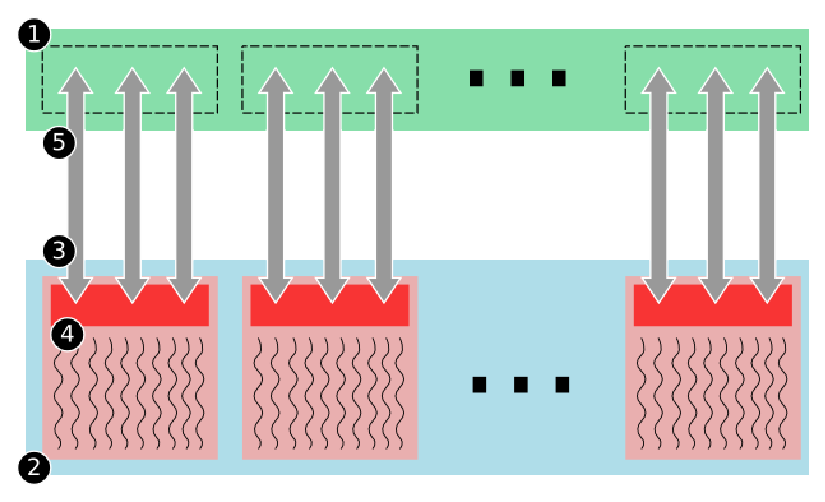
\includegraphics[width=0.9\textwidth]{img/cuda-strategy}
                \label{fig:estrategia}
                \caption{CUDA Programming strategy}
            \end{figure}
        \end{column}
        \begin{column}{0.5\textwidth}
             \begin{enumerate}
                 \item CPU memory allocation,
                 \item \dgreen{GPU} memory allocation,
                 \item Data copying,  CPU $\rightarrow$ \dgreen{GPU},
                 \item Task execution on the data,
                 \item Data copying, \dgreen{GPU} $\rightarrow$ CPU,
             \end{enumerate}
        \end{column}
    \end{columns}
\end{frame}

\subsection{Computational aspects}
\begin{frame}
    \frametitle{Computational Aspects}
    \framesubtitle{The computational challenge}

    \begin{itemize}
        \item The {\nbody} codes evolution is related to the available
                \blue{hardware} in our time.
        \item The algorithms with a complexity of $O(N^{2})$ or $O(N^{3})$ require
                \red{supercomputers}.
        \begin{itemize}
            \item  e.g \blue{beowulf clusters},
                which require a parallelization of the code
                (\textsc{Nbody6++} developed by Spurzem et al.~\cite{Spurzem1999}).

            \item Special-purpose hardware, like the \blue{GRAPE} (short for GRAvity
                PipE system~\cite{TMFES96,MT98,Makino98,GRAPE6A}.
        \end{itemize}

        \item  The literature overview reveals a strong interest on porting the existing codes to the
            \blue{GPU} architecture, like e.g. the work
            of~\cite{Portegies2007a,Hamada2007,Belleman2008}
            on single nodes or using large
            clusters~\cite{berczik2011high,NitadoriAarseth2012,Capuzzo-DolcettaEtAl2013}.

    \end{itemize}

\end{frame}

\subsubsection{CPU approach}
\begin{frame}
    \frametitle{Computational Aspects}
    \framesubtitle{Parallel CPU implementation}
    \begin{itemize}
        \item Single-core implementation to perform a profiling (\texttt{gprof}).
        \begin{itemize}
            \item Gravitational interaction is the bottleneck.
            \item Usually $N_{act} << N$.
        \end{itemize}
        \item Many-core with OpenMP.
        \begin{itemize}
            \item \soft{\texttt{\#pragma omp parallel for}}
        \end{itemize}
        \item Many-core with MPI (two implementations)
        \begin{itemize}
            \item \soft{\texttt{MPI\_Allreduce, MPI\_Bcast}}
        \end{itemize}
    \end{itemize}
\end{frame}

\begin{frame}[fragile]
    \frametitle{Computational Aspects}
    \framesubtitle{Parallel CPU implementation}

    \begin{columns}
        \begin{column}{0.45\textwidth}
            \begin{lstlisting}[language=C,caption={Reduce every $Nact$ particle}]
for (int i = 0; i < Nact; i++)
{
    ...
    for (int j = 0; j < N; j++)
    {
        gravitational_interaction(...);
    }
    ...
    MPI_Allreduce(...);
}
            \end{lstlisting}
        \end{column}
        \begin{column}{0.45\textwidth}
            \begin{lstlisting}[language=C,caption={Reduce all $Nact$ particle}]
for (int i = 0; i < Nact; i++)
{
    ...
    for (int j = 0; j < N; j++)
    {
        gravitational_interaction(...);
    }
    ...
}
MPI_Allreduce(...);
            \end{lstlisting}
        \end{column}
    \end{columns}
\end{frame}

\subsubsection{GPU Computing}
\begin{frame}
    \frametitle{Computational Aspects}
    \framesubtitle{GPU Computing}

    \begin{columns}
        \begin{column}{0.6\textwidth}
            \begin{center}
                \emph{"Using a GPU (Graphic Processing Unit) together with
                a CPU to accelerate scientific calculation operations
                or general purpose calculation"}
            \end{center}
        \end{column}
        \begin{column}{0.4\textwidth}
             \begin{figure}
                 \centering
                 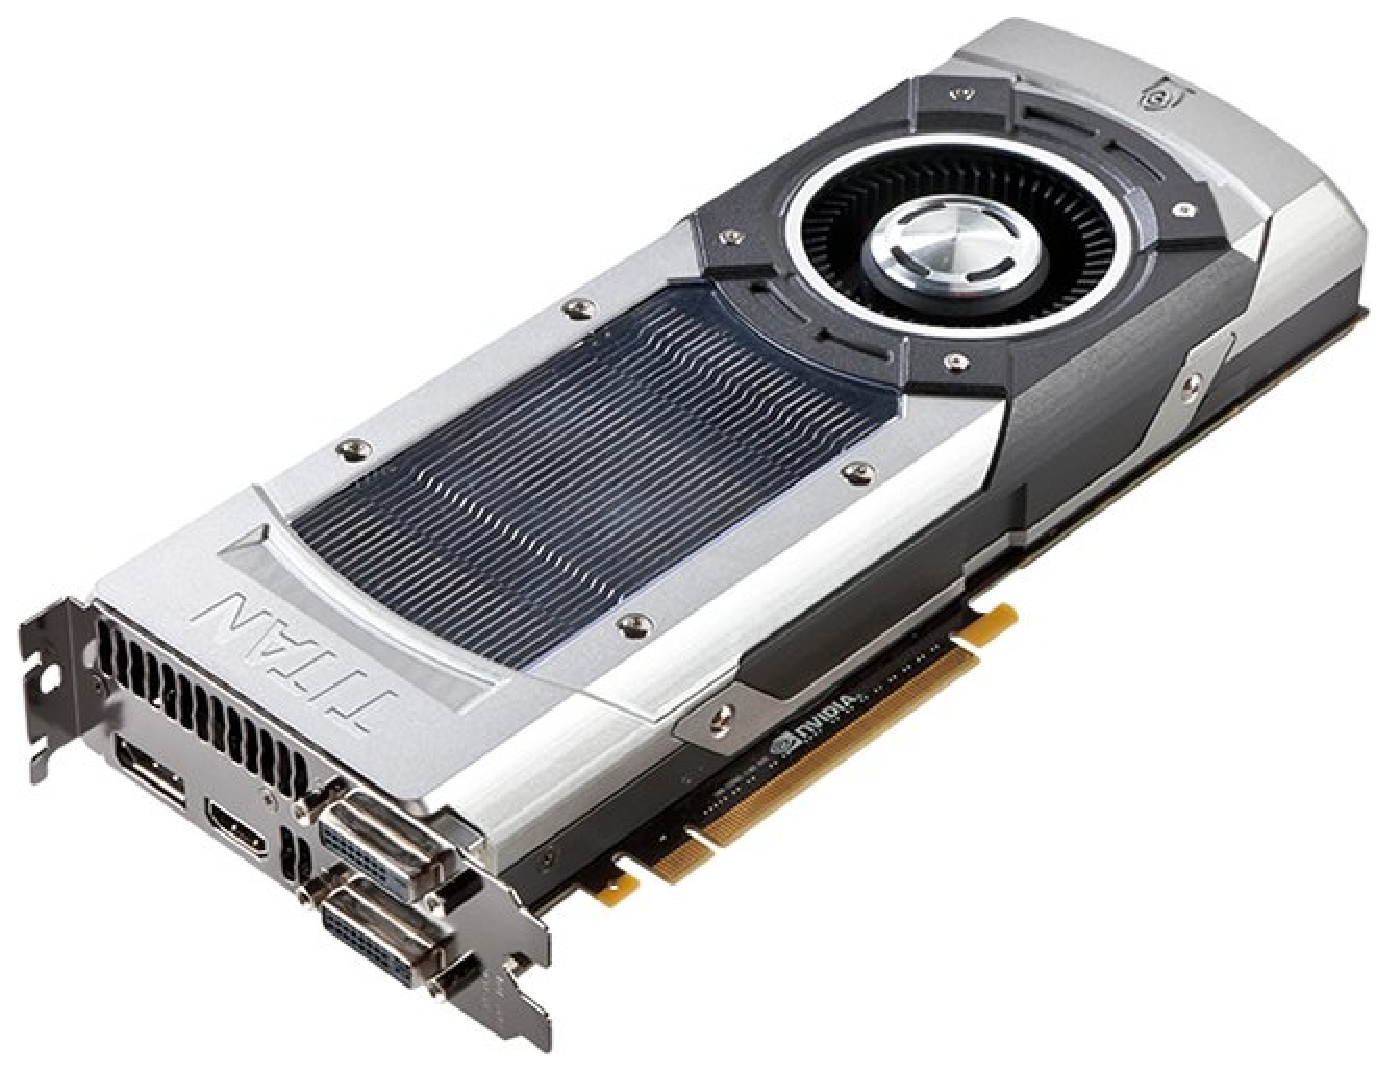
\includegraphics[width=0.8\textwidth]{img/titan}
                 \caption{NVIDIA\textsuperscript{\textregistered} GTX Titan}
                 \label{fig:titan}
             \end{figure}
        \end{column}
    \end{columns}
\end{frame}

\begin{frame}
    \frametitle{Computational Aspects}
    \framesubtitle{CPU/GPU Design}

    \begin{itemize}
        \item CPU,
        \begin{itemize}
            \item Designed to have a good \blue{performance}
                  in parallel and non-parallel scenarios.
            \item Minimizes the \blue{latency} experimented by a thread
                  (large cache memory)
        \end{itemize}
        \item GPU,
            \begin{itemize}
            \item Designed to perform highly parallel work.
            \item Maximizes the \blue{throughput} of all the threads.
            \end{itemize}
    \end{itemize}

    \begin{footnotesize}
        \begin{columns}
            \begin{column}{0.35\textwidth}
            \begin{block}{Performance}
                Capacity of perform individual instructions in a certain time.
            \end{block}
            \end{column}
            \begin{column}{0.3\textwidth}
            \begin{block}{Latency}
                Measure of time delay experienced in a system.
            \end{block}
            \end{column}
            \begin{column}{0.3\textwidth}
            \begin{block}{Throughput}
                Capacity of perform a whole task in a certain time.
            \end{block}
            \end{column}
        \end{columns}
    \end{footnotesize}
\end{frame}

\begin{frame}
    \framesubtitle{Computational Aspects}
    \frametitle{GPU Architecture}

    \begin{columns}
        \begin{column}{0.5\textwidth}
            \begin{block}{Task parallelism}
                Each processor perform a different task.
            \end{block}
            \begin{block}{Data parallelism}
                Each processor perform the same task, but not on the same data set.
            \end{block}
        \end{column}
        \begin{column}{0.5\textwidth}
             \begin{figure}
                 \centering
                 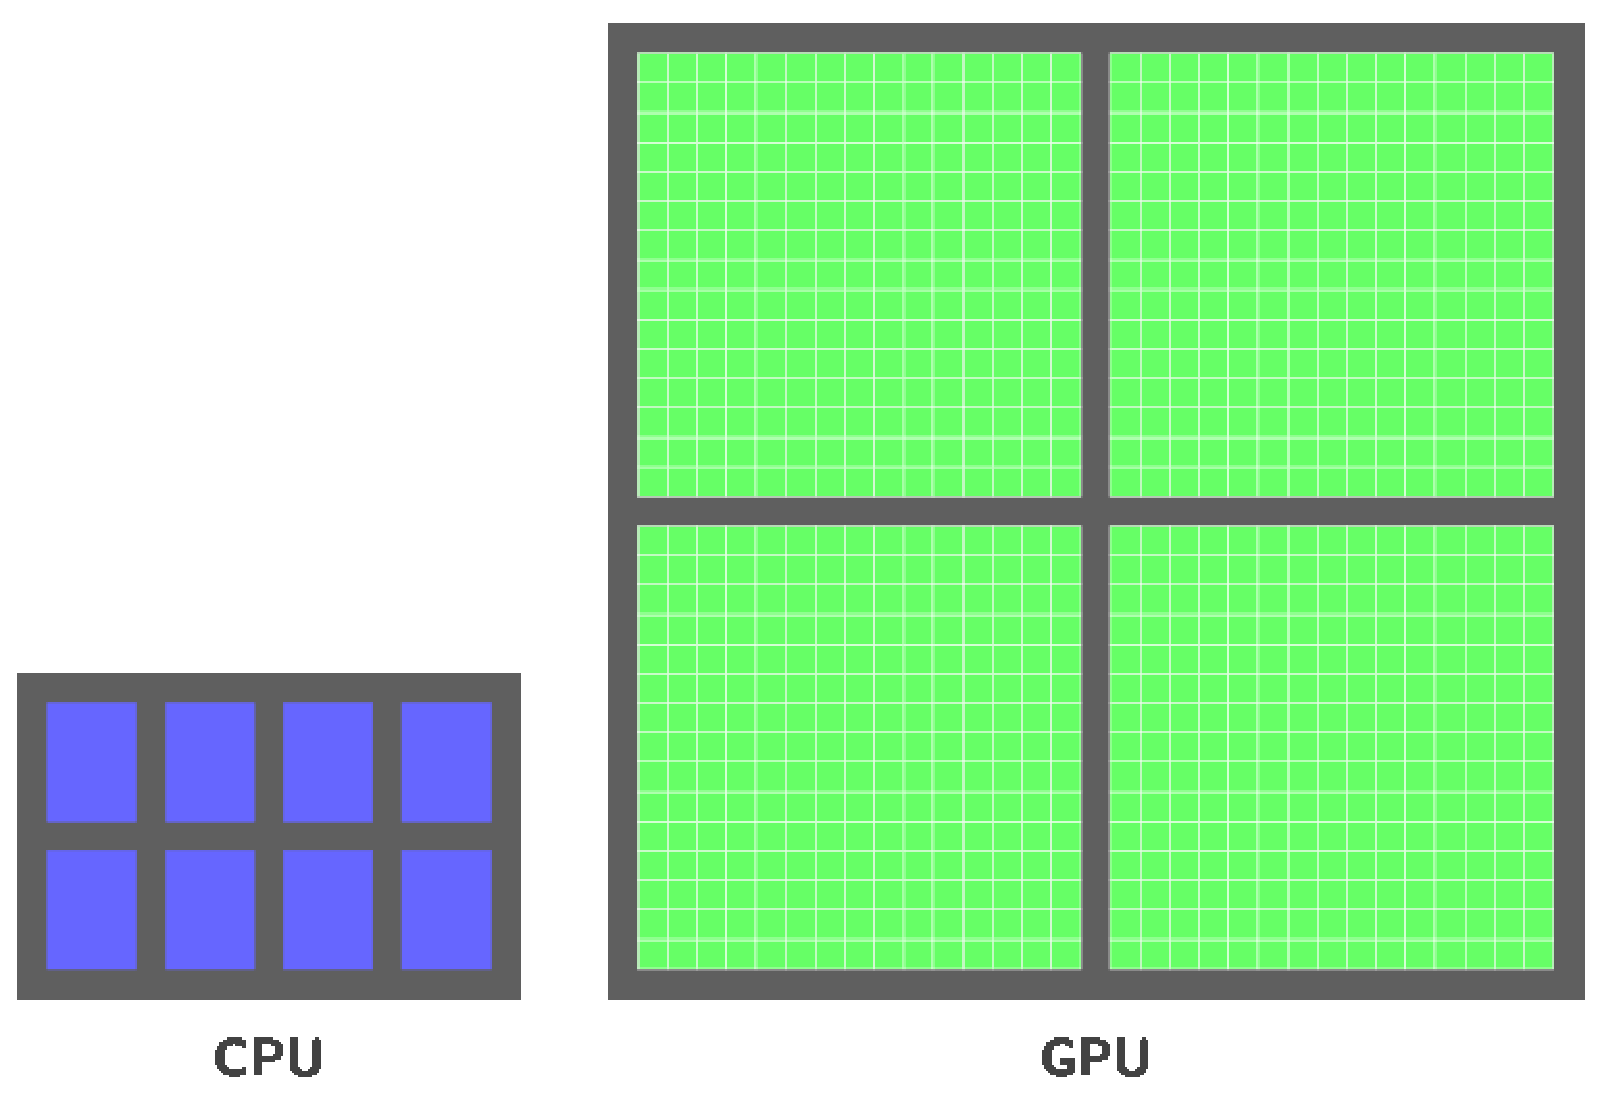
\includegraphics[width=0.8\textwidth]{img/cpu_gpu}
                 \caption{GPU and CPU core scheme}
                 \label{fig:core-scheme}
             \end{figure}
        \end{column}
    \end{columns}
\end{frame}

\subsubsection{Programming strategy}
\begin{frame}
    \frametitle{Computational Aspects}
    \framesubtitle{Programming strategy}

    \begin{columns}
        \begin{column}{0.5\textwidth}
            \begin{figure}
                \captionsetup{singlelinecheck=off}
                \centering
                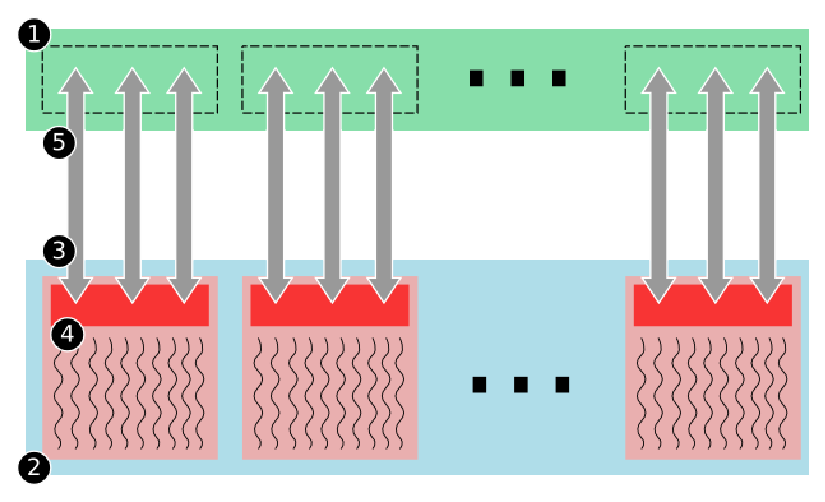
\includegraphics[width=0.9\textwidth]{img/cuda-strategy}
                \label{fig:estrategia}
                \caption{CUDA Programming strategy}
            \end{figure}
        \end{column}
        \begin{column}{0.5\textwidth}
             \begin{enumerate}
                 \item CPU memory allocation,
                 \item \dgreen{GPU} memory allocation,
                 \item Data copying,  CPU $\rightarrow$ \dgreen{GPU},
                 \item Task execution on the data,
                 \item Data copying, \dgreen{GPU} $\rightarrow$ CPU,
             \end{enumerate}
        \end{column}
    \end{columns}
\end{frame}

\begin{frame}
    \frametitle{Implementation}
    \framesubtitle{Integrators details}

    %\begin{columns}
    %    \begin{column}{0.5\textwidth}
            \begin{itemize}
                \item The code structure,
                \item Integration scheme,
                \item Parallelization scheme.
            \end{itemize}
    %    \end{column}

    %    \begin{column}{0.5\textwidth}
    %        \begin{Huge}
    %            \GR
    %        \end{Huge}
    %    \end{column}

    %\end{columns}

\end{frame}

%%%%%%%%%%%%%%%%%%%%%%%%%%%%%%%%%%%%%%%%%%%%%%%% CODE
%\section{The \GR\ code}
%\label{sec:code}
%\input{src/code}

\begin{frame}
    \frametitle{Implementation}
    \framesubtitle{The code}

    \begin{itemize}
        \item Main goal in the development, \blue{legibility}.
        \begin{itemize}
            \item Easy to read, modify and understand,
        \end{itemize}
        \item \blue{Balance} between optimization and maintainability.
    \end{itemize}


\end{frame}


\begin{frame}
    \frametitle{Implementation}
    \framesubtitle{The code}

    For the development of \GR, we have followed the next steps:

    \begin{itemize}
        \item Serial implementation,
        \item Profiling and performance assessment,
        \item Parallelization of the hot-spots,
        \item Optimization,
    \end{itemize}

    \begin{block}{\red{Note}}
        The same as CUDA C Best Practices~\cite{cudaBestPractices},
        called the APOD cycle, (Assess, Parallelize, Optimize and Deploy).
    \end{block}
\end{frame}


\begin{frame}
    \frametitle{Implementation}
    \framesubtitle{The code}

    \begin{itemize}
        \item OOP and SoA.
        \item Double-precision, importance of accuracy.
        \begin{itemize}
            \item on GPU, this reach the half of the theoretical maximum performance peak.
            \item NVIDIA Tesla C2050/M2050, single precision peak in GFLOPs is $1030.46$,
            and only $515.2$ with double precision.
        \end{itemize}
    \end{itemize}

    \begin{block}{\red{Note}}
        A posible future upgrade is to use mixed-precision~\cite{Aarseth85},
        or pseudo double-precision~\cite{keigo} to achieve a better performance
        in our code.
    \end{block}

\end{frame}

%%%%%%%%%%%%%%%%%%%%%%%%%%%%%%%%%%%%%% Integration scheme
%\section{Integration scheme}
%\label{sec:hermite}
%\input{src/hermite}

\begin{frame}
    \frametitle{Prediction-correction method}
    \framesubtitle{Introduction}
    \begin{columns}
        \begin{column}{0.6\textwidth}
            \begin{block}{In a {\nbody} system}
                The force acting on each particle varies smoothly.
            \end{block}

            \begin{itemize}
                \item Interpolation for the time interval extension (prediction).
                \item Reduce the amount of the force calculation.
                \item By finite differences it is possible to get the higher order
                derivatives of the force, which are used to add precision (correction).
            \end{itemize}
        \end{column}
        \begin{column}{0.4\textwidth}
            \begin{figure}
                \centering
                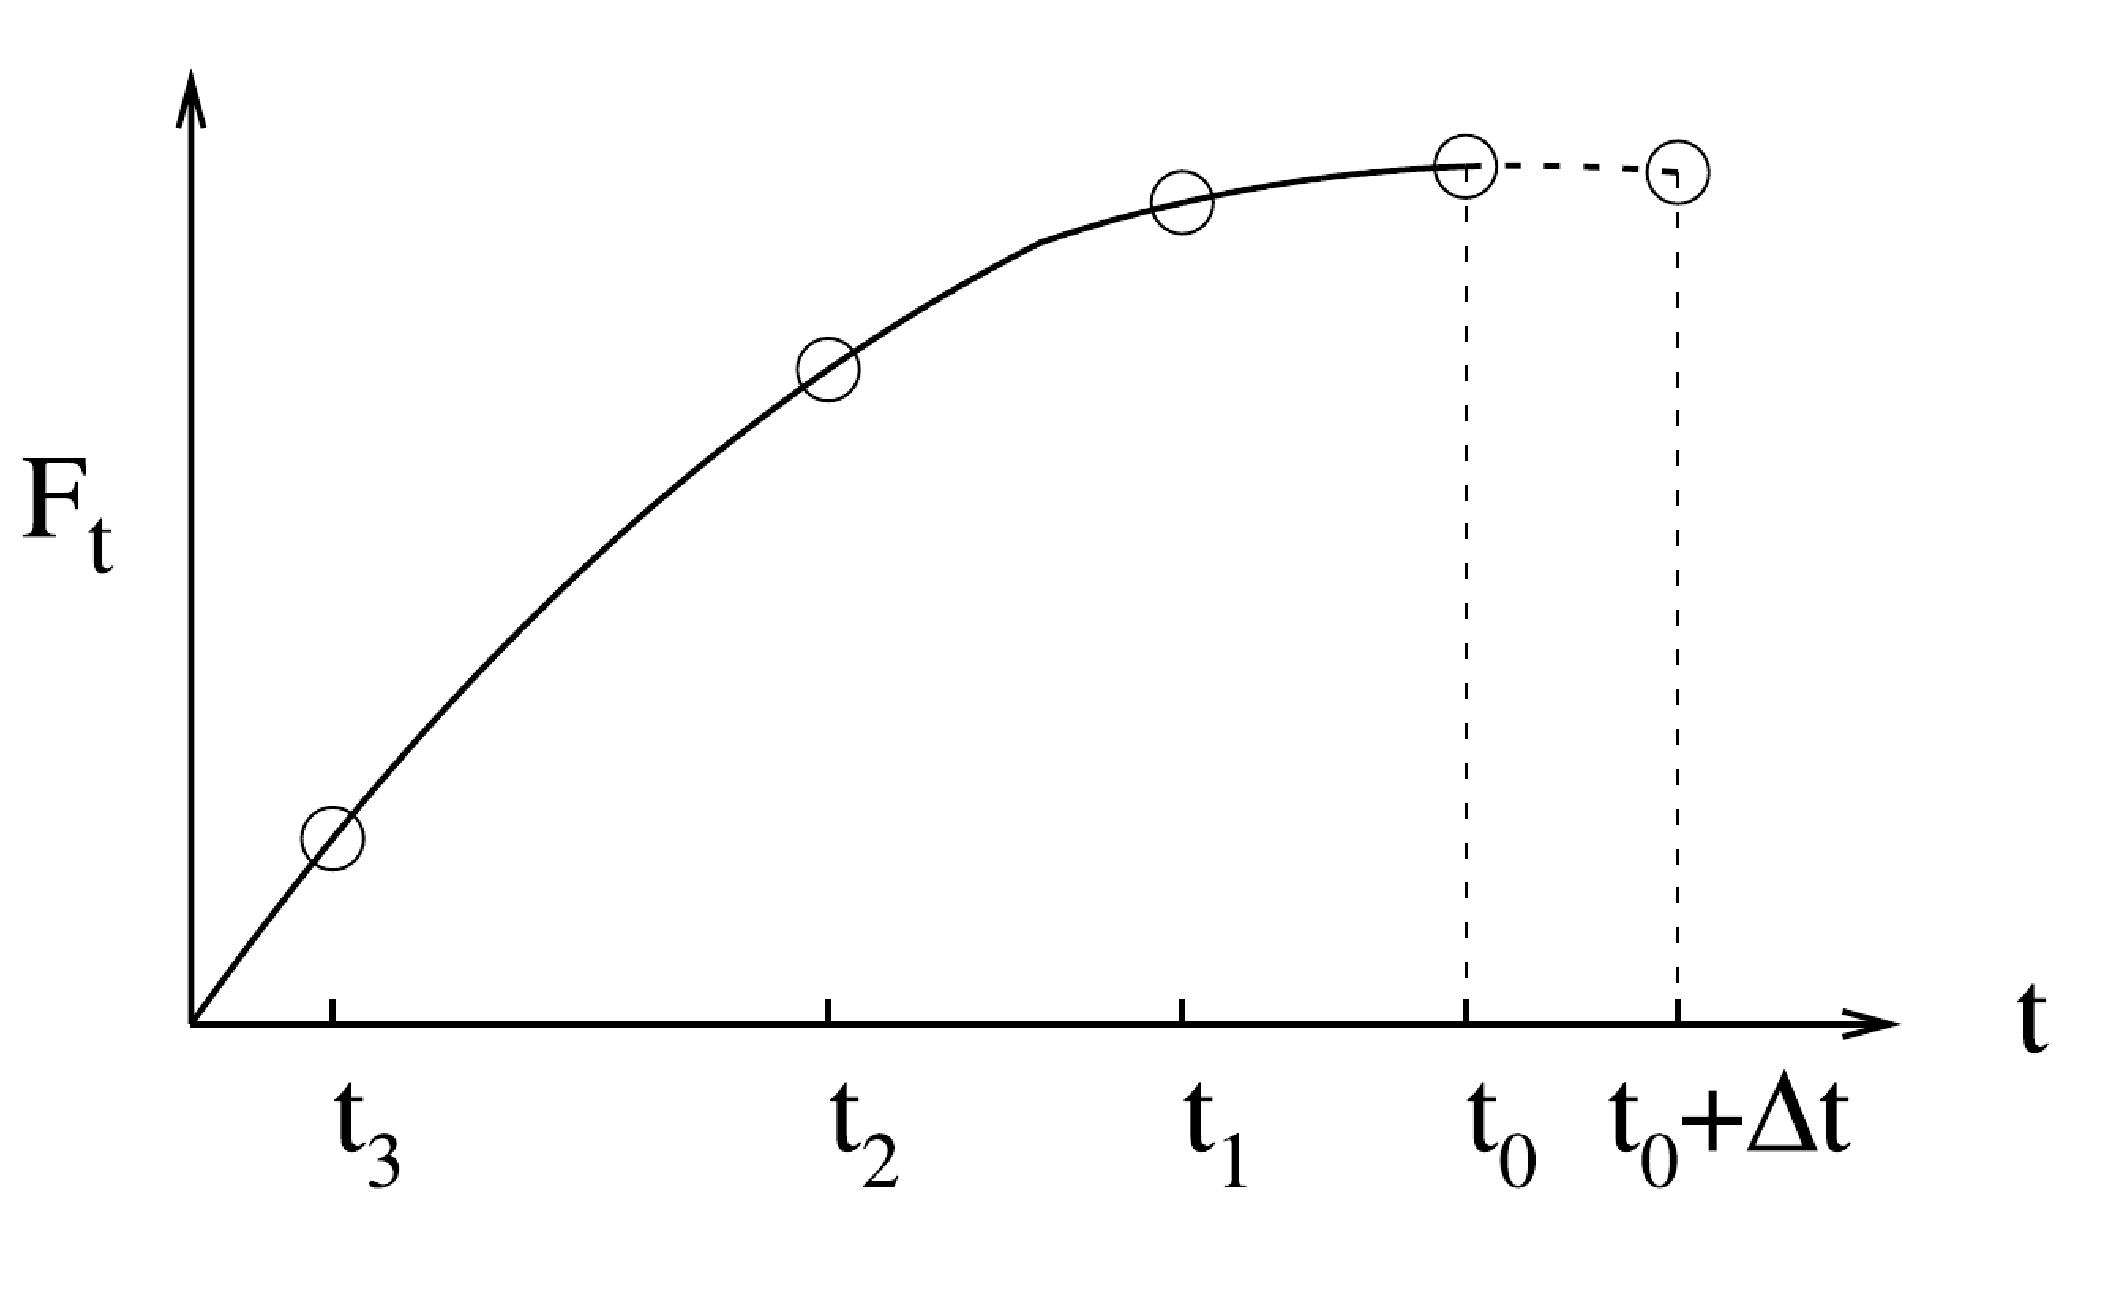
\includegraphics[width=0.8\textwidth]{img/polinomio}
                \caption{Polynomial fit of the gravitational force in function of time.}
                \label{fig:polinomio}
            \end{figure}

        \end{column}
    \end{columns}
\end{frame}

\begin{frame}[fragile]
    \frametitle{Prediction-correction method}
    \framesubtitle{Block time steps}
    \begin{columns}
        \begin{column}{0.6\textwidth}
            \begin{itemize}
                \item Reduce the amount of predictions,
                \item Enhance the parallelism,
                \item Based on an adaptive system.
                \begin{footnotesize}
                    \begin{dmath}
                        \Delta t_{i} = \sqrt{\eta  \frac{|\bs{a}_{i}|
                                                             |\bs{a}_{i}^{(2)}| +
                                                             |\bs{a}^{(1)}_{i}|^{2}}
                                                            {|\bs{a}^{(1)}_{i}|
                                                             |\bs{a}_{i}^{(3)}| +
                                                             |\bs{a}_{i}^{(2)}|^{2}}
                                                },\\
                    \end{dmath}
                \end{footnotesize}
            \end{itemize}

            \begin{small}
                \begin{block}{Block definition}
                    $2^{n} \Delta t_{s} \leq \Delta t_{i}\ $\textless$\ 2^{n+1} \Delta t_{s}$
                \end{block}
            \end{small}
        \end{column}
        \begin{column}{0.4\textwidth}
            \begin{figure}
                \centering
                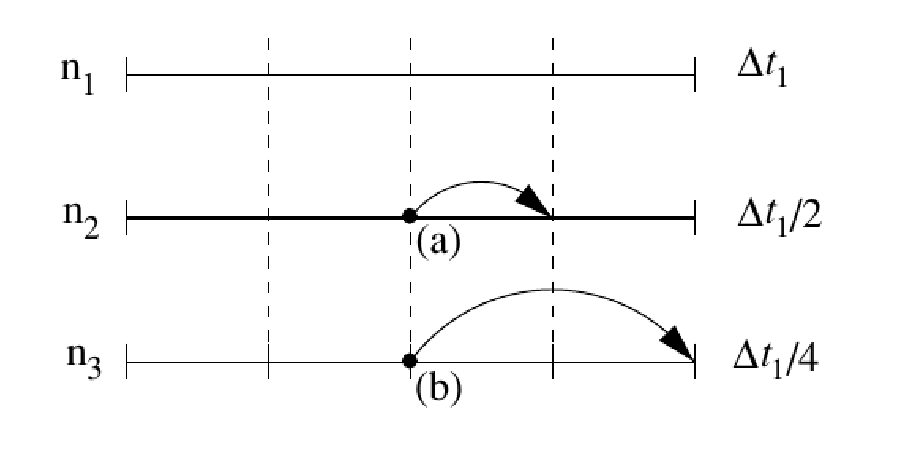
\includegraphics[width=0.9\textwidth]{img/blockdt}
                \caption{Time step hierarchical levels.}
                \label{fig:blockdt}
            \end{figure}
        \end{column}
    \end{columns}
\end{frame}

\begin{frame}
    \frametitle{Prediction-correction method}
    \framesubtitle{Hermite scheme}
    \begin{columns}
        \begin{column}{0.5\textwidth}
        \begin{block}{Prediction}
        \footnotesize
        \begin{dmath}
            \bs{r}_{i,pred} = \bs{r}_{i,0} +
                            \bs{v}_{i,0} \Delta t_{i}  +
                            \frac{1}{2!} \bs{a}_{i,0} \Delta t^{2}_{i} +
                            \frac{1}{3!} \bs{\dot{a}}_{i,0} \Delta t^{3}_{i}
        \end{dmath}
        \begin{dmath}
            \bs{v}_{i,pred} = \bs{v}_{i,0} +
                            \bs{a}_{i,0} \Delta t_{i}  +
                            \frac{1}{2!} \bs{\dot{a}}_{i,0} \Delta t^{2}_{i}
        \end{dmath}

        \end{block}
        \end{column}
        \begin{column}{0.5\textwidth}
            \begin{figure}
                \centering
                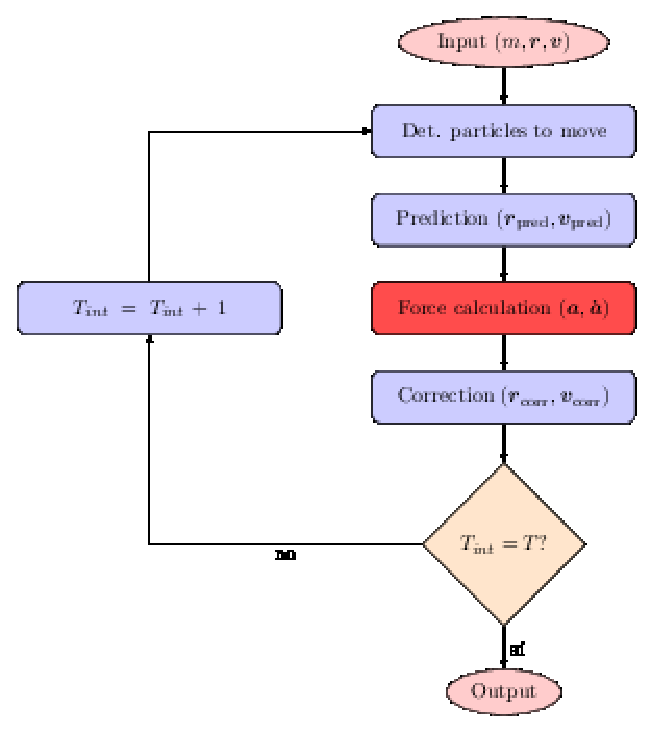
\includegraphics[height=0.7\textheight]{diagrams/algorithm}
                %\caption{}
                \label{fig:algoritmo}
            \end{figure}
        \end{column}
    \end{columns}
\end{frame}


\begin{frame}
    \frametitle{Prediction-correction method}
    \framesubtitle{Hermite scheme}
    \begin{columns}
        \begin{column}{0.5\textwidth}
            \begin{block}{Force calculation}
                \footnotesize
                \begin{dmath}
                    \bs{a}_{i,1} = \sum_{\substack{j=0\\j\neq i}}^{N} G m_{j}
                                    \frac{\bs{r}_{ij}}
                                           {(r_{ij}^2 + \epsilon^{2})^{\frac{3}{2}}}, \\
                \end{dmath}
                \begin{dmath}
                    \bs{\dot{a}}_{i,1} = \sum_{\substack{j=0\\j\neq i}}^{N} G m_{j}
                                    \left[
                                        \frac{\bs{v}_{ij}}
                                            {(r_{ij}^2 + \epsilon^{2})^{\frac{3}{2}}} -
                                        \frac{3(\bs{v}_{ij}\cdot \bs{r}_{ij}) \bs{r}_{i}}
                                            {(r_{ij}^2 + \epsilon^{2})^{\frac{5}{2}}}
                                    \right],
                \end{dmath}
            \end{block}
        \end{column}
        \begin{column}{0.5\textwidth}
            \begin{figure}
                \centering
                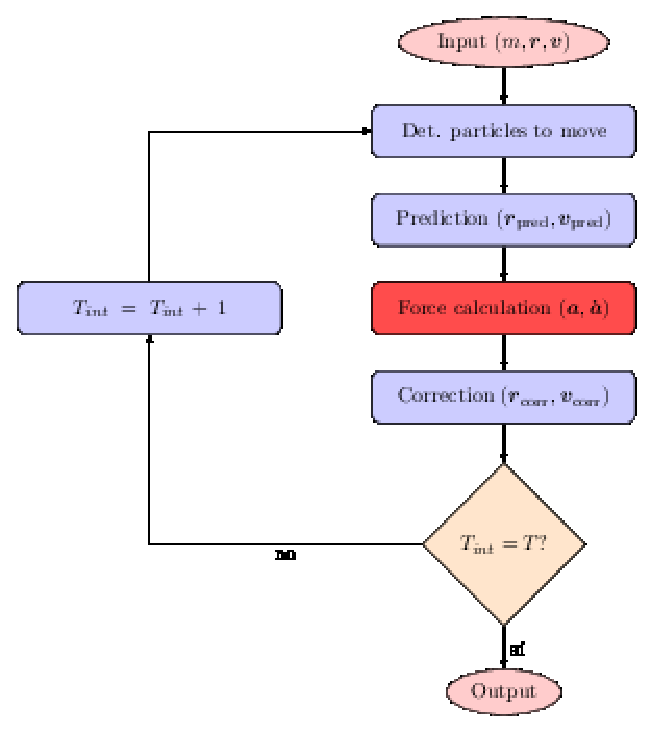
\includegraphics[height=0.7\textheight]{diagrams/algorithm}
                %\caption{}
                \label{fig:algoritmo}
            \end{figure}
        \end{column}
    \end{columns}
\end{frame}

\begin{frame}
    \frametitle{Prediction-correction method}
    \framesubtitle{Hermite scheme}
    \begin{columns}
        \begin{column}{0.5\textwidth}
        \begin{block}{Correction}
        \small
        \begin{dmath}
            \bs{r}_{i,1} = \bs{r}_{i,pred} +
                                \frac{1}{24}  \Delta t_{i}^{4} \bs{a}_{i,0}^{(2)} +
                                \frac{1}{120} \Delta t_{i}^{5} \bs{a}_{i,0}^{(3)} \\
        \end{dmath}
        \begin{dmath}
            \bs{v}_{i,1} = \bs{v}_{i,pred} +
                                \frac{1}{4}  \Delta t_{i}^{3} \bs{a}_{i,0}^{(2)} +
                                \frac{1}{24} \Delta t_{i}^{4} \bs{a}_{i,0}^{(3)}
        \end{dmath}

        \end{block}
        \end{column}
        \begin{column}{0.5\textwidth}
            \begin{figure}
                \centering
                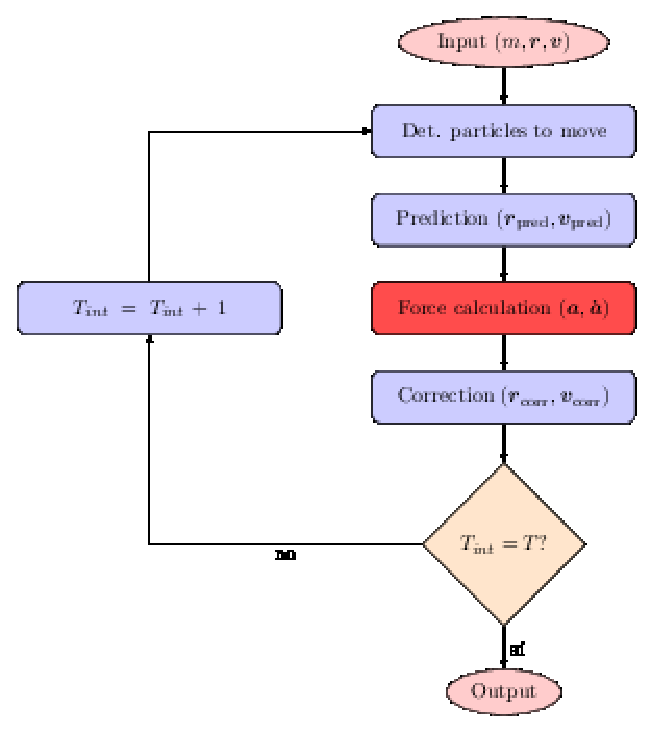
\includegraphics[height=0.7\textheight]{diagrams/algorithm}
                %\caption{}
                \label{fig:algoritmo}
            \end{figure}
        \end{column}
    \end{columns}
\end{frame}


%%%%%%%%%%%%%%%%%%%%%%%%%%%%%%%%%%%%%%%%%%%%%%%%%%%%%
%\section{The parallelization scheme}
%\label{sec:parallel}
%\input{src/parallel}

\begin{frame}
    \frametitle{Parallelization scheme}
    \framesubtitle{Force calculation}

    \begin{center}
    \begin{figure}[H]
        \centering
        \includegraphics[width=0.6\textwidth]{img/force_calculation.pdf}
        \caption{Force calculation code illustration.
                 The process itself belongs to a second level \texttt{for} loop.
                 Thanks to the integrator scheme, we have a reduction
                 of the step complexity from $O(N^{2})$ to $O(N_{act} N)$}
        \label{fig:force_code_diagram}
    \end{figure}
    \end{center}

\end{frame}

\begin{frame}
    \frametitle{Parallelization scheme}
    \framesubtitle{Calculation relations}

    \begin{center}
    \begin{figure}[H]
        \centering
        \includegraphics[width=0.7\textwidth]{img/forces_nact_n.pdf}
        \caption{Relation between the particles which will be updated in a certain
                 integration time ($N_{\rm act}$) and the whole set of particles ($N$).
                 The relation between the active particles and the others is
                 $N_{\rm act} << N$}
        \label{fig:nact_n}
    \end{figure}
    \end{center}

\end{frame}

\begin{frame}
    \frametitle{Parallelization scheme}
    \framesubtitle{Threads task}

    \begin{center}
    \begin{figure}[H]
        \centering
        \includegraphics[width=0.6\textwidth]{img/force_nact.pdf}
        \caption{For each $i-$particle in $N_{\rm act}$ a \texttt{for} will be through
                 the whole set of particles and perform the calculation of the
                 gravitational interaction between $i$ and $N$ particles.
                 The scheme could be know as $i-$parallelization, since it assumes
                 that each thread will be one $N_{\rm act}$
                 particle.}
        \label{fig:force_nact}
    \end{figure}
    \end{center}

\end{frame}

\begin{frame}
    \frametitle{Parallelization scheme}
    \framesubtitle{Tiles scheme}

    \begin{center}
    \begin{figure}[H]
        \centering
        \includegraphics[width=0.45\textwidth]{img/tiles.pdf}
        \caption{Grid configuration using the \emph{tiles} approach (This figure
        is based on~\cite{gpuGems3})}
        \label{fig:tile}
    \end{figure}
    \end{center}

\end{frame}

\begin{frame}
    \frametitle{Parallelization scheme}
    \framesubtitle{$j-$parallelization scheme}

    Our configuration is based in the idea presented in~\cite{NitadoriAarseth2012},

    \begin{center}
    \begin{figure}[H]
        \centering
        \includegraphics[width=0.55\textwidth]{img/force_split_reduction.pdf}
        \caption{Parallelization scheme to split the $j-$loop instead of the $i-$loop.
                 In this case, we have two sections, the first is to calculate
                 the force interactions of the $i-$particle with the whole
                 system but by different threads. Then a reduction (sum) is necessary
                 to get the new value for the $i-$particle force.}
        \label{fig:force_split_reduction}
    \end{figure}
    \end{center}

\end{frame}


\section{Experiments}
\begin{frame}
    \frametitle{Experiments}
    \framesubtitle{Details of the hardware}

    \begin{center}
        \begin{tabular}{lr}
            \hline
            {CPU} & Intel(R) Xeon(R) CPU E5-4650 0 @ 2.70GHz \\
            {GPU} & Tesla M2050 @ 575 Mhz (448 cores). \\
            {RAM} & 24 GB \\
            {OS}  & Scientific Linux release 6.4 \\
            \hline
        \end{tabular}
    \end{center}
\end{frame}

\begin{frame}
    \frametitle{Experiments}
    \framesubtitle{Integrator scaling}

\begin{figure}[H]
    \centering
    \label{fig:time}
    \includegraphics[width=0.65\textwidth]{img/test_time-1t-N.pdf}
    \caption{Clock time of integration from $t=1$ to $t=2$ NBU using $\eta = 0.01$ and
             $\epsilon = 10^{-4}$ using different amount of particles.}
\end{figure}

\end{frame}

\begin{frame}
    \frametitle{Experiments}
    \framesubtitle{Clock time comparison}

\begin{table}[H]
    \centering
    \footnotesize
    \begin{tabular}{rrrrrrr}
        \hline
        {\bf N} & \multicolumn{1}{c}{\bf CPU}
                & \multicolumn{1}{c}{\bf OpenMP}
                & \multicolumn{1}{c}{\bf CPU + GPU}
                & \multicolumn{1}{c}{\bf MPI-1}
                & \multicolumn{1}{c}{\bf MPI-2}
                & \multicolumn{1}{c}{\bf GPU}   \\
         %{\bf  1k} &    12.98 [s] &     8.19 [s]  &    3.57 [s]      &    6.17 [s] &    2.68 [s] &    1.21 [s]          \\
         %{\bf  2k} &    61.32 [s] &    34.94 [s]  &   13.42 [s]      &   14.51 [s] &    7.34 [s] &    3.22 [s]          \\
         %{\bf  4k} &   282.98 [s] &   162.64 [s]  &   54.28 [s]      &   51.14 [s] &   27.12 [s] &    9.45 [s]          \\
         %{\bf  8k} &  1227.40 [s] &   682.56 [s]  &  208.91 [s]      &  105.65 [s] &   64.61 [s] &   23.31 [s]          \\
         %{\bf 16k} &  5542.35 [s] &  3227.91 [s]  &  904.82 [s]      &  364.90 [s] &  317.51 [s] &   82.63 [s]          \\
         %{\bf 32k} & 26383.71 [s] & 15076.40 [s]  & 3722.92 [s]      & 1247.33 [s] & 1145.82 [s] &  275.53 [s]          \\ \hline
         {\bf  1k} &    12 &     8  &    3      &    6  &    2 &    1          \\
         {\bf  2k} &    61 &    34  &   13      &   14  &    7 &    3          \\
         {\bf  4k} &   282 &   162  &   54      &   51  &   27 &    9          \\
         {\bf  8k} &  1227 &   682  &  208      &  105  &   64 &   23          \\
         {\bf 16k} &  5542 &  3227  &  904      &  364  &  317 &   82          \\
         {\bf 32k} & 26383 & 15076  & 3722      & 1247  & 1145 &  275          \\ \hline
    \end{tabular}
    \caption{Clock time foreach integrator version (in sec).}
    \label{tab:acc}
\end{table}

\end{frame}

\begin{frame}
    \frametitle{Experiments}
    \framesubtitle{Clock time comparison}

\begin{figure}[H]
    \centering
    \label{fig:acc}
    \includegraphics[width=0.8\textwidth]{img/test_gpu-acceleration.pdf}
    \caption{Acceleration between the implementations described in Table~\ref{tab:acc}}
\end{figure}

\end{frame}
\begin{frame}
    \frametitle{Experiments}
    \framesubtitle{Integrator Performance}
\begin{figure}[H]
    \centering
    \label{fig:gflops}
    \includegraphics[width=0.65\textwidth]{img/test_gflops.pdf}
    \caption{GPU gravitational interactions performance in GFLOPS for different amount of particles.}
\end{figure}

\end{frame}

\section{Projects}
\begin{frame}
    \frametitle{Projects}
    \framesubtitle{Software}

    The current version of our new {\nbody} code,
    written in C/C++ and CUDA, called {\GR}.

    \begin{itemize}
        \item The current version of our code,
        \begin{itemize}
            \item Using \blue{Hermite 4th order} integration scheme.
            \item Block timesteps for helping parallelism.
            \item \blue{Suitable} in the energy conservation,
                reaching errors around $\approx 10^{-9}$ and $\approx 10^{-7}$-
            \item OO.
            \item Documentation (Doxygen).
        \end{itemize}
    \end{itemize}
\end{frame}

\begin{frame}
    \frametitle{Projects}
    \framesubtitle{Software development}

    \begin{itemize}
        \item Main software
        \begin{itemize}
            \item Main goal in the development, \blue{legibility}.
            \begin{itemize}
                \item Easy to read, modify and understand,
            \end{itemize}
            \item \blue{Balance} between optimization and maintainability.
        \end{itemize}
        \item Utility scripts.
    \end{itemize}
\end{frame}

\section{Future work}
\begin{frame}
    \frametitle{Projects}
    \framesubtitle{Milestones}

    \begin{itemize}
        \item Programming
        \begin{itemize}
            \item Multi-GPU environment, large clusters (MPI).
        \end{itemize}
        \item Physics
        \begin{itemize}
            \item Semi-Keplerian systems (BH).
            \item Neighbors treatment.
            \item Regularisations (KS, Chain, ...)
            \item Higher order integration schemes.
            \item Smoothed-particle hydrodynamics (SPH).
            \item ...
        \end{itemize}
    \end{itemize}
\end{frame}


% Final slide
\begin{frame}[t,plain]
\titlepage
\end{frame}

\begin{frame}[allowframebreaks]
\footnotesize
\bibliographystyle{ieeetr}            %
\bibliography{phdproject}
\end{frame}

\end{document}
